\chapter{Numerical implementation}

In this section we outline the details of the numerical solution of the equations. GKW uses a combination of finite difference and spectral methods.
The turbulence in the plane perpendicular to the magnetic field is homogeneous and the
solution in the $\zeta, \psi$ plane is represented by Fourier modes, as mentioned
previously. All other directions are treated using finite difference techniques.
In what follows $N_{\rm mod}$ and $N_x$ are the number of bi-normal ($\zeta$ direction) and radial ($\psi$ direction) modes
respectively, $N_{sp}$ is the number of kinetic species, $N_s$ the number of grid points along the field line. $N_{v\parallel}$ is the number of grid points 
in the parallel velocity direction and $N_\mu$ the number of magnetic moment grid points. 

\section{Derivatives along the magnetic field line and in the parallel velocity
direction}
\label{sec:finite-differences}
Terms I, IV and VII on the right hand side of \Eq{eqs:complete-set}, involving a derivative along the magnetic field line or in the parallel velocity direction are considered
here. These terms correspond to an advection with a spatially dependent advective velocity
and can be written in the form $-v(s)\frac{\partial g}{\partial s}$. The second and fourth-order centred-differences used for these
terms can then be written
% \label{general_advection}
%\end{equation}
\begin{equation} 
v {\partial g \over \partial s} \rightarrow v_i {- g_{i-1} + g_{i+1} \over 2 \Delta s} 
- D \vert v_i \vert {g_{i-1} - 2 g_i + g_{i+1} \over 2 \Delta s},
\label{eq:s-2nd-order}
\end{equation} 
\begin{align}
v {\partial g \over \partial s}  \rightarrow  v_i {g_{i-2} - 8 g_{i-1} + 8 g_{i+1} -g_{i+2} \over 
12 \Delta s}
 %\cr \noalign{\vskip 0.2 truecm} & &
 - D \vert v_i \vert {- g_{i-2} + 4 g_{i-1} - 6 g_i + 4 g_{i+1}-g_{i+2} \over 12 \Delta s},  
\label{eq:s-4th-order}
\end{align}
where the terms involving a dissipation coefficient $D$ correspond to (hyper)diffusive upwind dissipation. This dissipation is
not included in the case of term VII (containing derivatives of $\phi$) for numerical stability reasons.

\ifmoredetails Merely to keep the code simple, the finite difference
expression for the 4th derivative in \eq{s-4th-order} has only second
order accuracy, as a higher order would involve more than just 5
gridpoints.

The fact that in Fourier representation the $\partial_s^4$ becomes
$ik_s^4$ illustrates that the dissipation term affects in particular
the small scales.\\
Note that only a small dissipative contribution is desired, the
smaller the higher the grid resolution is. Hence it makes sense to
prepend the dissipation term with a factor $\Delta s^n$, where $n$ is
an arbitrary power. This should make an appropriate choice of the
coefficient $D$ (parameters \name{disp\_par} and \name{disp\_vp}) more
obvious.
\begin{align}
 - D \Delta s^n\vert v_i \vert {- g_{i-2} + 4 g_{i-1} - 6 g_i + 4 g_{i+1}-g_{i+2} \over 12 \Delta s^4}\nonumber
\end{align}
One may consider a grid-scale oscillation, i.e. $g_{i} = 1$ for even
indices $i$ and $-1$ for odd $i$. This is just the kind of oscillation
that the artifical dissipation term is supposed to suppress.  In this
example, the finite difference in the dissipation term yields
$1/\Delta s^4$ while that of the advection yields $1/\Delta s$.  If
one prepends the dissipation with $\Delta s^3$ then for coefficients
$D \sim 1$ the dissipation term is comparable to the advection term
and will indeed damp the grid-scale oscillation effectively. This is
why in \eq{s-4th-order} only $\Delta s$ appears, not $\Delta s^4$.
% For a large scale oscillation may be illustrated by
% $g_i = -2, -1, 0, 1, 2$ on five neighbouring points. Then the
% dissipation term yields $2 - 4 - 0 + 4 - 2=0$ while the advection
% gives $1/\Delta s$.
\fi

Rather than apply this central differencing scheme separately to terms I and IV, the code user can choose an
alternative scheme, which combines the derivative along the field line
with the trapping term. Defining $H(s,v_{\parallel}) = \frac{1}{2} v_{\parallel}^2 + \mu B+\frac{1}{2}{\cal E}_R$, and noting that
$B {\cal G} = {\cal F} {{\partial B}\over{\partial s}}$ in IV, we can combine terms
I and IV to give
\begin{equation}
\label{eq:arakawa}
v_R {\cal F} \bigg( \mu \frac{\partial B}{\partial s}\frac{\partial \hat{f}}{\partial v_{\parallel}}  -
v_{\parallel}\frac{\partial \hat{f}}{\partial s} \bigg) =
v_R {\cal F} ~\{H,\hat{f}\},
\end{equation}
where $\{H,\hat{f}\}$ is a Poisson bracket (note that we have neglected the redundant
dependence of $\mu$ in the definition of $H$ for simplicity). Following the second and
fourth-order schemes of Arakawa \cite{A66}, we allow the Poisson bracket to be
differenced directly. The terms containing $D$ in
\Eqs{eq:s-2nd-order}{eq:s-4th-order} are also added to allow some dissipation. The
advantage of this scheme over the separate differencing scheme is that usually zero (or relatively small) dissipation is
needed to obtain a stable solution. Presently this is implemented only as a fourth-order scheme.

\section{Boundary conditions along a field line}
We here discuss the implementation of the boundary conditions in the parallel direction $s$, that are presented in Sec.~\ref{sec:spectral}.
After one poloidal turn the Fourier mode connects to a mode with a different radial wave vector.
The grid in the $s$ direction is therefore constructed such that at the end of the field line it connects smoothly to 
the start of the field line (i.e. the grid spacing remains constant). Of course, the radial wave vector to which 
the mode has to connect might not be represented on the grid. At the end (or beginning) of the field line 
a boundary condition is then employed. GKW allows for a choice in this boundary condition, setting the 
perturbed distribution either to zero (NO LONGER AVAILABLE) or to have a zero derivative (default, \name{parallel_boundary_conditions='open'}) in the direction upwind with respect
to the convection.\footnote{The option \name{parallel_boundary_conditions='Dirichlet'} may be different to both of these and is experimental - not documented further here.} 
The down wind direction is always treated with a zero derivative boundary condition, allowing the distribution to 
'flow off the grid', without reflections. 
Close to the end point boundaries a staggered change in differencing order accuracy is used to remove 
ghost cells and to allow the flow of the distribution function out of the domain.  
Reflection or the allowed build up at the upper velocity boundaries is seen as unphysical and therefore undesirable.  
Because of the use of up-winding the boundary condition is dependent on the sign of the advective velocity.

When the advective velocity $v(s)$ is positive the distribution function will move toward the left boundary, and the 
following scheme is used
\begin{eqnarray}
\mbox{Boundary cell}: & & \mbox{Second order scheme} - \frac{\partial g}{\partial s} \rightarrow \frac{-\frac{3}{2}g_{n} + 2g_{n+1} -\frac{1}{2}g_{n+2}}{\Delta s},\nonumber\\
\mbox{Adjacent cell}: & & \mbox{Third order} - \frac{\partial g}{\partial s} \rightarrow \frac{-\frac{1}{3}g_{n-1} -\frac{1}{2}g_{n} + g_{n+1} - \frac{1}{6}g_{n+2}}{\Delta s}. \nonumber
\end{eqnarray}
with the right hand boundary using the centrally differenced schemes.  
When the advective velocity is negative the opposite is true and the right hand boundary is differenced in an identical way.  
To obtain the scheme for the opposing boundary simply reverse the signs of the equation above.
When using the second order scheme, special consideration is needed only for the boundary cell.  
Depending on the direction of the advective velocity, a first order back-winded scheme is used at the boundary. 
The effect of these open boundary conditions is to remove the need for ghost cells in the differencing scheme while maintaining 
a high order scheme. 
Compared to other alternatives we have found that the chosen scheme removes rapid fluctuations near the end points, and 
therefore allows for a minimum dissipation. In the Poisson bracket formulation \eq{arakawa}, the above convention is integrated into the scheme at the boundaries to have similar properties. Less (or no) dissipation (Diffusion/super-diffusion) is needed for this scheme, but the dissaption is implemented as separate routine using the normal differencing above, allowing identical dissipation to be applied to both schemes.

\begin{figure}
\begin{center}
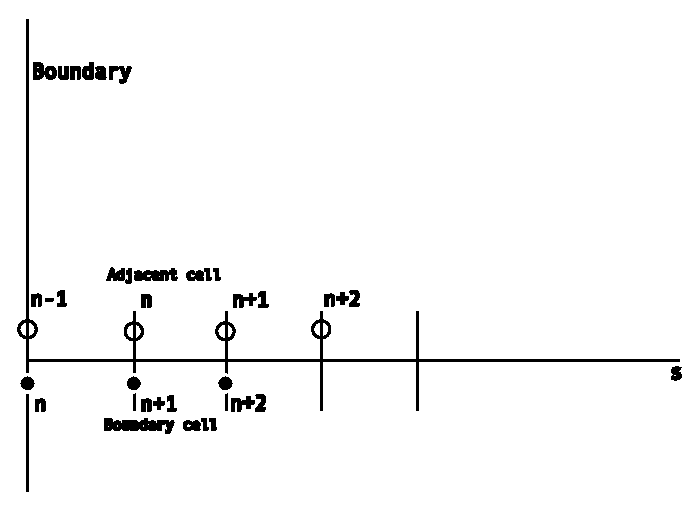
\includegraphics[width=0.5\textwidth]{Boundarydiff.eps}
\caption{Schematic showing the cells of intest in the differencing scheme when considering the boundary cell (Hollow circles) and the adjacent cell (Filled circles).  The figure shows the left hand boundary, for right hand simply reflect in the y direction}
\label{boundarydiffs}
\end{center}
\end{figure}

% Does new refer to zero-deriv and old to zero ?
\begin{figure}
\begin{center}
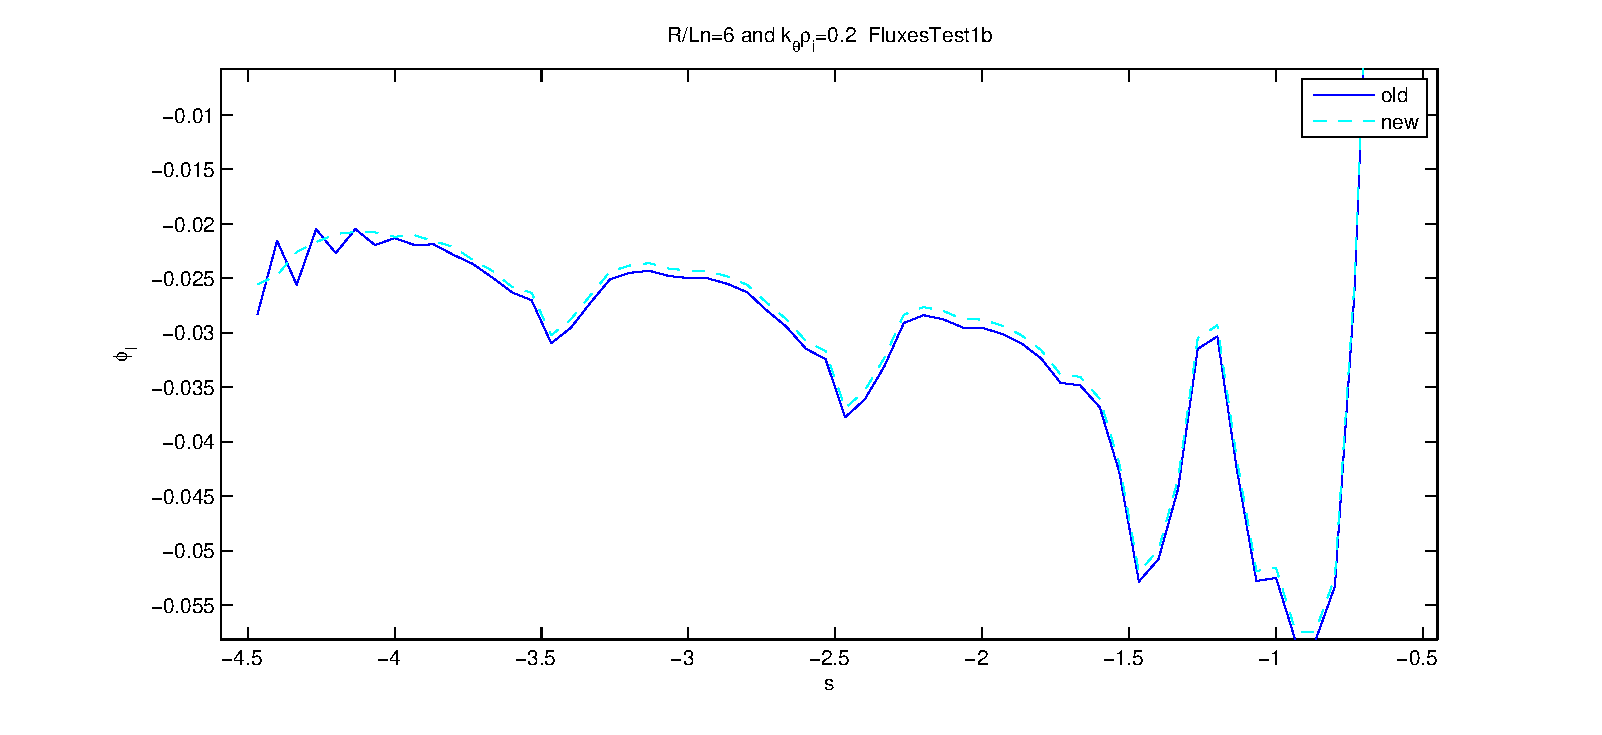
\includegraphics[width=0.5\textwidth]{fluxcomp.eps}
\caption{Figure showing the effect of the new open boundary conditions at the boundary. The new boundary has reduced cell to cell fluctuations giving a smoother solution.}
\label{fluxcomp}
\end{center}
\end{figure}

\noindent


The effect of the open boundary conditions is to remove the need for ghost cells in the differencing scheme while maintaining a high order scheme. It has reduced the amplitude of cell to cell fluctuations refelecting off the boundary (See figure \ref{fluxcomp}), which in turn, has reduced the need for adding artificial dissipation to the system to damp away these modes.  The dissipation, however, can not be wholly turned off in non-linear runs.  Note also that the dealiasing in nonlinear runs also has some dissipative effect in the perpendicular spatial directions.

\section{Parallel velocity grid - Trapping condition} %Added by Will 29/6/2008
(STILL EXPERIMENTAL AND UNDER DEVELOPMENT)
By contorting the velocity grid to conform to the electron trapping condition we are able to remove terms that involve derivatives in the parallel velocity direction.  This greatly speeds up linear run computation times but more significantly removes the need for numerical diffusion in the parallel velocity direction and lastly, provides resolution in the required areas.

This option is turned on by setting \name{vp\_trap} $= 1$ in the \name{CONTROL} namelist of the input deck.  A further parameter is needed in the \name{GRIDSIZE} namelist which is named \name{n\_trapped} which is the number of grid points within the trapped region of the velocity grid.

In the current implementation of the trapping condition, the number of cells in the s direction and the number of points in the parallel velocity direction add certain restrictions to the number of points that can be placed within the trapped region.

Firstly, for ease of differencing the bounce points of a specific $v_{\parallel 0}$ (The velocity on the low-field side) must occur exactly half way between two grid-cells, thus the number of grid cells in the s direction restrict both the number and initial values of $v_{\parallel}$.  The maximum number of bounce points available is given by \name{n\_s\_grid}$/2 - 1$.  The value of \name{n\_trapped} must be less than or equal to this.  If less is chosen then the code will select which points to use determined by the spacing between points (The closer to the boundary, the closer the bounce points become), the algorithm will iterate over the points, sequentially removing points until \name{n\_trapped} are left.  \name{n\_trapped} must also be less than \name{n\_vpar\_grid}.  Outside the trapping region the points are uniformly placed, the spacing is determined by the number \name{n\_vpar\_grid} $- 2\times$ \name{n\_trapped}.

\begin{figure}[h!]
\begin{center}
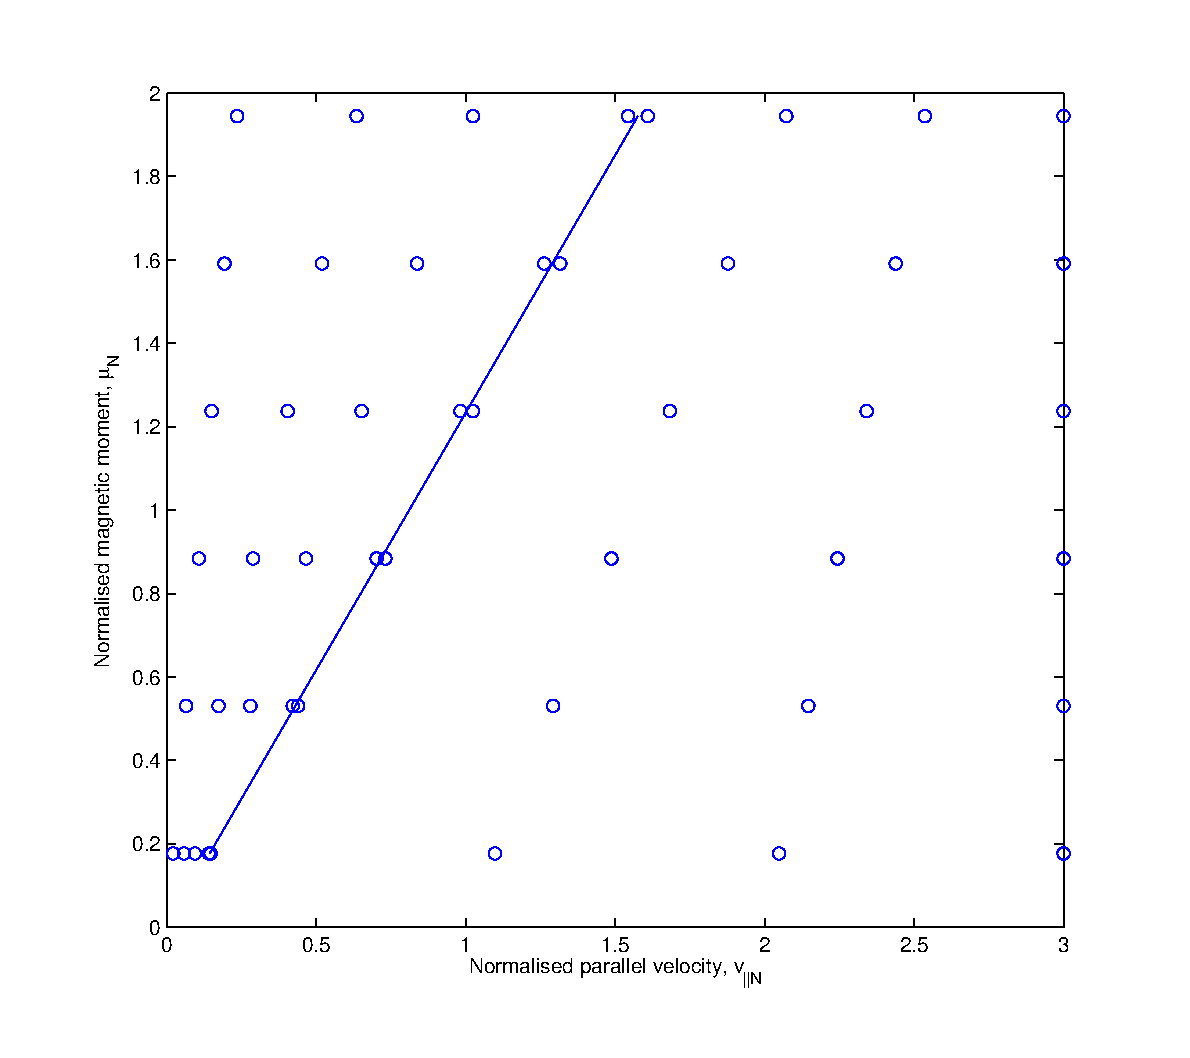
\includegraphics[width=0.4\textwidth]{traplowfield.eps}
\caption{Figure of parallel velocity grid points as given by the trapping condition, the line corresponds to the trapped/untrapped boundary $v_{||0} = \sqrt{2\mu(B_{max}-B_{min})+\cfen^{H}-\cfen^{L}}$.  In the above data, N_vpar_grid $= 16$ (only one half of the grid is shown as it is symmetric),n_trapped $= 4$ and $\mu = 6$. It must be noted that the total number of points within the trapped region (full grid) is $2\times$n_trapped.}
\label{lowfieldsidetrap}
\end{center}
\end{figure}

This algorithm gives the grid at the low field side (For an example see figure \ref{lowfieldsidetrap}), this is then propagated around the torus by the equation
\begin{equation}
v_{\parallel N} = \sqrt{v_{\parallel 0 N}^{2} + 2\mu_{N}(B - B_{0}) + \cfen- \cfen^{\rm L}}
\end{equation}
\noindent
where $B_{0}$ is the magnetic field at the low field side, and $\cfen^L$ is the centrifugal energy at the low field side.  When a bounce point is reached, the velocity becomes zero, and all velocity grid points after this along $s$ are set to zero and are ignored in the differencing.  The grid is also symmetric around $v_{\parallel}=0$.


Rules that must be followed, otherwise the code will throw you out,
\begin{itemize}
\item The value of \name{n\_trapped} must be less than \name{n\_vpar\_grid}/2
\item \name{n\_trapped} must also be less than or equal to \name{n\_s\_grid}/2$-1$
\item For optimal convergence $2\times$\name{n\_trapped} must be roughly half of \name{n\_vpar\_grid}. (This may no longer be true: See \issue{8} for latest updates on Gaussian integration (and section \ref{sec:gaussian-integration})
\end{itemize}

\section{Gaussian Integration}
\label{sec:gaussian-integration}

This is a short note on how the Gaussian integration is implemented in GKW. 

We wish to calculate the integral over the normalized parallel velocity $v_\parallel$ 
\begin{equation}
I = \int\nolimits_{v_{tp}}^{v_{pm}} g(v_\parallel) {\rm d} v_\parallel 
\end{equation} 
The integral is over (half of the) passing domain with the lower limit the trapped-passing 
boundary ($v_{tp}$) which is a function of $\mu$. We use Gaussian integration 
in combination with ${\rm vp\_trap = 1}$, in which case the parallel velocity grid must 
satisfy 
\begin{equation} 
v_{\parallel k}^2 = v_{\parallel 0}^2 + 2 \mu (B_0 - B_k) 
\end{equation} 
where $v_{\parallel k}$ is the parallel velocity at grid point k along the magnetic field, 
with $B_k$ being the local magnetic field, and the index 0 indicates the low field 
side position. We can therefore define only one set of parallel velocity gird points 
with the grid at different locations along the field line satisfying the equation 
above. The integral is therefore written in low field side coordinates 
\begin{equation} 
I = \int\nolimits_{v_{pt0}}^{v_{pm0}} g(v_\parallel ( v_{\parallel 0}) ) {{\rm d} v_\parallel \over 
{\rm d} v_{\parallel 0}} \biggr \vert_\mu \, {\rm d} v_{\parallel 0} 
\end{equation} 
From the relation between $v_\parallel$ and $v_{\parallel 0}$ it follows 
\begin{equation} 
{{\rm d} v_\parallel \over {\rm d} v_{\parallel 0}} \biggr \vert_\mu  = {v_{\parallel 0} \over 
v_\parallel } 
\end{equation}
We furthermore choose to write $g$ as 
\begin{equation}
{v_{\parallel 0} \over v_\parallel} g = \exp [-v_{\parallel 0}^2 ] z(v_{\parallel 0} )
\label{zdef} 
\end{equation} 
This choice is of course motivated by the expected dependence of $g$ on $v_\parallel$. The 
Maxwellian background will lead to the strong exponential decay. It is this exponential 
dependence that we would like to 'transform away' in order to obtain an efficient integration
algorithm. 

With the choices discussed above the integral is 
\begin{equation}
I = \int\nolimits_{v_{tp0}}^{v_{pm0}} \exp [ - v_{\parallel 0}^2 ] z(v_{\parallel 0}) {\rm d} v_{\parallel 0} 
\end{equation} 
Using the transformation 
\begin{equation} 
y = {\rm erf} (v_{\parallel 0}) \qquad {\rm with}\qquad {\rm erf}(v_{\parallel 0} ) = {2 \over \sqrt{\pi}} 
\int_0^{v_{\parallel 0}} \exp [-x^2] {\rm d} x
\end{equation} 
one obtains 
\begin{equation} 
I = {\sqrt\pi \over 2 } \int\nolimits_{ya}^{yb} z(y(v_{\parallel 0})) {\rm d} y 
\end{equation} 
with 
\begin{equation} 
ya = {\rm erf}(v_{tp0}) \qquad yb = {\rm erf}(v_{pm0} ) 
\end{equation} 
Finally, we transform the integral to the interval [-1,1], using the transformation 
\begin{equation} 
\alpha = {2 y \over yb - ya} - {ya + yb \over yb - ya} 
\end{equation} 
to obtain 
\begin{equation} 
I = {1\over 4} \sqrt\pi (yb - ya) \int_{-1}^1 z(\alpha(y)) {\rm d} \alpha 
\end{equation} 
The latter integral can then be solved by a standard Gauss Legendre integration using the points 
$\alpha_i$ and weights $w_i$ (which can be obtained from publicly available software) 
\begin{equation} 
\int_{-1}^1 z(\alpha(y)) {\rm d} \alpha = \sum\nolimits_{i = 1}^m  w_i z(\alpha_i) 
\end{equation} 

For the implementation we transform back to $v_{\parallel}$ 
\begin{equation} 
I = {1 \over 4} \sqrt\pi (yb-ya) \sum\nolimits_{i = 1}^m w_i \exp[ + v_{\parallel 0i}^2] {v_{\parallel 0 i} \over v_\parallel (v_{\parallel 0i} ) } 
g(v_\parallel(v_{\parallel 0i})) 
\end{equation} 
with the points of the grid $v_{\parallel 0 i}$ determined by the relation 
\begin{equation} 
{\rm erf}(v_{\parallel 0 i} ) = ya + (yb - ya)(\alpha_i + 1 )/2 
\end{equation}



\section{The collision operator}
\label{numerics:collisions}
The collision operator can be thought of as a convection/diffusion equation in velocity space and thus is differenced accordingly.
The velocity space boundary conditions are taken to be zero flux, which occurs naturally at the $\mu =0$ boundary and is artificially
imposed on the other three boundaries.  These boundary conditions guarantee the conservation of mass.  
Considering that the diffusion coefficient is velocity space dependent, and the grid can be non-uniform in the $\mu$-direction, the differencing scheme of the equations is chosen as follows for the parallel velocity direction
\begin{equation}
\frac{\partial}{\partial v_\parallel}\left(D\frac{\partial \hat{f}}{\partial v_{\parallel}}\right) \rightarrow
\frac{1}{v_{i+1/2\parallel}^{j}-v_{i-1/2\parallel}^{j}}\Big( D_{i+1/2}^{j}\left(\frac{f_{i+1}^{j}-f_{i}^{j}}{v_{i+1\parallel}^{j}-v_{i\parallel}^{j}}\right) - 
D_{i-1/2}^{j}\left(\frac{f_{i}^{j}-f_{i-1}^{j}}{v_{i\parallel}^{j}-v_{i-1\parallel}^{j}}\right)\Big),
\end{equation}
\noindent
where i denotes the point in the parallel velocity direction and j the $\mu$ direction.  When considering the cross-terms a four point 
interpolation method is used to calculate the half point values.  Four points are needed on a two-dimensional grid.
The friction term is differenced in the same way, but with a two point interpolation.  

To bypass the complications caused by non-uniform distribution of $\mu$ points (which in uniform in the $v_\perp$ coordinate), the code chooses the suitable version of the
collision operator that is uniform, and as such, can conserve mass (and parallel momentum) to machine accuracy.  

A further switch \textbf{selfcollcon} in the collisions input deck changes the momentum conservation from just the self-collisions for each species (selfcollcon = .true.) to absolute conservation (selfcollcon=.false, default=.true.). Note that the absolute conservation option is unphysical and only implemented for tests and benchmarks purposes.

\section{The Fourier representation} 

In a nonlinear run a rectangular grid of wave vectors ($k_\zeta,k_\psi$) is used. 
The nonlinearity is treated using fast Fourier transforms (FFT).
Different choices of FFT libraries are possible, but at present we use mostly the FFTW library \cite{FFT05}. 
For the nonlinear term a de-aliasing method is applied, i.e. the transformation to real space is constructed on a grid finer 
(number of grid points at least 3/2 larger in real space) than the Fourier modes represent. 
The de-aliasing method is non-conservative and has a dissipative effect on the finer grid scales, with the consequence that a 
numerical dissipation term in the spectral directions is generally not required.

Since the distribution function is a real quantity the number of
complex Fourier modes can be reduced by a factor two and a half plane
of wavevectors with $k_\zeta \ge 0$ is used.  Grid sizes in real space
are chosen so that they have only small prime factors. Such sizes lead
to particularly efficient computations with the standard FFT
libraries. There are no significantly more efficient grid sizes any
more, as it used to be in the past.

\section{Time integration}

GKW has several options for the explicit time integration: modified midpoint, fourth order Runga Kutta (recommended), 
and a second order scheme that is stable for hyperbolic equations. An implicit scheme is also implemented, but is still under development
and not yet recommended for general use (For latest updates see \issue{10}). 

\section{Poisson equation \label{Poisson-detail}}

The Poisson equation \ref{Poisson-adiabatic} is split into three linear terms which are stored in 
the main solution matrix,  but evaluated separately from the other linear terms. 
The calculation of the fields takes place in \File{fields.F90} subroutine \name{calculate_fields}.

The Poisson equation given in \ref{Poisson-adiabatic} can be rewritten.
\ifmoredetails
\begin{align}
  &\sum_{sp , ions }  Z_{sp} n_{R_0,sp} \biggl [ 
  2 \pi B \int {\rm d} v_{\parallel} {\rm d} \mu J_0(k_\perp\rho_{sp}) \hat g_{sp} + {Z_{sp} \over T_{Rsp}} [ \Gamma(b_{sp}) -1]\exp(-\cfennsp{sp}) \hat \phi 
  \biggr ] =  { n_{R_0,e}\exp(-\cfennsp{e})
    \over T_{Re}} ( \hat \phi - {\fsa{\hat \phi }}) \nonumber\\
  &
  \sum_{sp , ions }  Z_{sp} n_{R_0,sp} \biggl [ 
  2 \pi B \int {\rm d} v_{\parallel} {\rm d} \mu J_0(k_\perp\rho_{sp}) \hat g_{sp}
  \biggr ]
  + { n_{R_0,e}\exp(-\cfennsp{e}) \over T_{Re}} {\fsa{\hat \phi }} 
  = {} \nonumber\\
  &\qquad {} = 
  -\sum_{sp , ions }  Z_{sp} n_{R_0,sp} \biggl [ 
  {Z_{sp} \over T_{Rsp}} [ \Gamma(b_{sp}) -1]\exp(-\cfennsp{sp}) \hat \phi 
  \biggr ]
  + { n_{R_0,e}\exp(-\cfennsp{e}) \over T_{Re}} \hat \phi
 \nonumber\\
\end{align}
Solving for $\hat\phi$
\begin{align}
  &
  \sum_{sp , ions }  Z_{sp} n_{R_0,sp} \biggl [ 
  2 \pi B \int {\rm d} v_{\parallel} {\rm d} \mu J_0(k_\perp\rho_{sp}) \hat g_{sp}
  \biggr ]
  + { n_{R_0,e}\exp(-\cfennsp{e}) \over T_{Re}} {\fsa{ \hat\phi}} 
  = {} \nonumber\\
  &\qquad {} = 
  \left[-\sum_{sp , ions }  Z_{sp} n_{R_0,sp} \biggl [ 
  {Z_{sp} \over T_{Rsp}} [ \Gamma(b_{sp}) -1]\exp(-\cfennsp{sp})
  \biggr ]
  + { n_{R_0,e}\exp(-\cfennsp{e}) \over T_{Re}} \right] \hat \phi
 \nonumber\\
\end{align}
yields
\fi
\begin{align}
\hat{\phi }= -{1 \over A} \left[ \sum_{sp , ions }  \underbrace{Z_{sp} n_{R_0,sp} 2 \pi B \int {\rm d} v_{\parallel} {\rm d} \mu J_0(k_\perp\rho_{sp})}_{\name{poisson_int()}\rightarrow M^3} \hat g_{sp} + \underbrace{{n_{Re}\exp(-\cfennsp{e}) \over T_{Re}}
 \fsa{\hat\phi}}_{\name{poisson_zf()}\rightarrow \text{eq. \ref{eq:zonalmatrixform}}}
\right]
\label{eq:poisson2}
\end{align}
where the factor
\begin{equation}
 A =  \sum_{\rm sp, ions} n_{sp} Z_{sp} \left[ {Z_{sp} \over T_{Rsp}} ( \Gamma(b_{sp}) -1)\exp(-\cfennsp{sp}) - {\exp(-\cfennsp{e}) \over T_{Re} } \right] = M^4
\end{equation}
is evaluated in subroutine \name{poisson_dia}. The symbols $M^3$ and
$M^4$ number the matrices presented in this paragraph (and are not
``powers of $M$'' or so) and refer to sections of \name{mat}. In this
sense also $M^1$ and $M^2$ which contain the linear terms of the GKE
and are mentioned elsewhere denote sections 1 and 2 of the matrix
\name{mat}. The quantity $\fsa{\hat\phi}$ can be eliminated from
\ref{eq:poisson2} by taking the flux surface average of equation
\ref{eq:poisson2}.  
\ifmoredetails
\begin{align}
\fsa{\hat{\phi}} &= \fsa{-{1 \over A} \left[ 
    \sum_{sp , ions }  Z_{sp} n_{R_0,sp} 2 \pi B \int {\rm d} v_{\parallel} {\rm d} \mu J_0(k_\perp\rho_{sp}) \hat g_{sp} 
    + {n_{Re}\exp(-\cfennsp{e}) \over T_{e}} \fsa{\hat \phi}
  \right]} \nonumber\\
 &= \fsa{-{1 \over A} 
    \sum_{sp , ions }  Z_{sp} n_{R_0,sp} 2 \pi B \int {\rm d} v_{\parallel} {\rm d} \mu J_0(k_\perp\rho_{sp}) \hat g_{sp} 
    }
    + \fsa{-{1 \over A}{n_{Re}\exp(-\cfennsp{e}) \over T_{Re}} \fsa{\hat \phi}  
}
\end{align}
The expressions containing $\fsa{\hat\phi}$ are drawn together:
\begin{align}
\fsa{\hat\phi} - \frac{n_{Re}}{T_{Re}}\fsa{\frac{-\exp(-\cfennsp{e})}{A}} \fsa{\hat \phi}
  &= \fsa{-{1 \over A} 
    \sum_{sp , ions }  Z_{sp} n_{R_0,sp} 2 \pi B \int {\rm d} v_{\parallel} {\rm d} \mu J_0(k_\perp\rho_{sp}) \hat g_{sp} 
}\nonumber
\end{align}
\begin{align}
\fsa{\hat\phi}\left(
  1
  -
  \frac{n_{Re}}{T_{Re}}\fsa{\frac{-\exp(-\cfennsp{e})}{A}}\right)
  &=\nonumber\\
\frac{n_{Re}}{T_{Re}}\exp(-\cfennsp{e})\fsa{\hat\phi}\left(
  \frac{T_{Re}}{n_{Re}}\frac{1}{\exp(-\cfennsp{e})}
  -
  \fsa{\frac{-1}{A}}\right)
  &=
\end{align}
\fi
The zonal correction term can then be written as a function of the
distribution function, parameters and background quantities.
\begin{align}
{n_{Re}\exp(-\cfennsp{e}) \over T_{Re} } \fsa{\hat\phi}
&= { \fsa{
-{1 \over A} \sum_{sp, ions}  Z_{sp} n_{R_0,sp} 2 \pi B \int {\rm d} v_{\parallel} {\rm d} \mu J_0(k_\perp\rho_{sp})\hat g_{sp}
}
 \over
 {1 \over \exp(-\cfennsp{e})} \left({T_Re \over n_Re} + \fsa{{\exp(-\cfennsp{e}) \over A}}\right)} 
\label{eq:zonal}
\end{align}
The subroutine \name{poisson_zf} prepares matrices according to the definitions
\begin{align}
  Z &= -\frac{\ud s}{A} \\
  Y &= \frac{1}{\exp(-\cfennsp{e})} \left({T_Re \over n_Re} + \fsa{{\exp(-\cfennsp{e}) \over A}}\right)
\end{align}
which are used to express the right hand side of \ref{eq:zonal} in the form
\begin{align}
{n_{Re}\exp(-\cfennsp{e}) \over T_{Re} } \fsa{\hat\phi}
  &= {\sum_s Z M^3 {\hat g} \over Y}\ .
\label{eq:zonalmatrixform}
\end{align}
\ifmoredetails
Thanks to \ref{eq:zonal}, \ref{eq:poisson2} allows the subroutine
\name{calculate_fields} to calculate $\hat\phi$ explicitely.
\begin{align}
\hat{\phi } & = \sum_s Z M^3 {\hat g} + {\sum_s Z M^3 {\hat g} \over Y} \\
            & = {(Y + 1)\sum_s Z M^3 {\hat g} \over Y}\ .
\end{align}
\fi


To calculate $\hat\phi$ from the distribution function, first the integral
part \name{poisson_int} is evaluated using section $M^3$ of the
matrix.
\begin{equation}
a_i(k_y,k_x,s) = M^{3}_{ij} {\hat g}_j.
\end{equation}
Next, the zonal flow correction term, equation \ref{eq:zonal}, is evaluated
separately, using the special ``matrices'' $Z$ and $Y$.  First, the flux surface
average in the numerator is evaluated.
\begin{equation}
b_i(k_x) = \sum_s Z_{ij} a_j 
\end{equation}
Then each element is divided by the denominator from equation \ref{eq:zonal}.
\begin{equation}
c_i(0,k_x,s)) = b_i / Y_i(s) 
\end{equation}
The zonal correction term is then subtracted from the minuend in
equation \ref{eq:poisson2}.
\begin{equation}
d_i(k_y,,k_x,s)=a_i-c_i 
\end{equation}
Finally, all elements are divided by the factor $A$ ($A$ being identical
to $M^4$, the section 4 of ``the matrix of the linear terms'').
\begin{equation}
{\hat \phi}_i(k_y,k_x,s) = d_i / M^4_i
\end{equation}
The other linear terms are stored in sections 1 and 2 of the matrix and evaluated as 
$\hat{f_i}^\prime = \hat{f_i} + \delta t \cdot \hat{f_j} M^{1,2}_{ij}$ in \name{calculate_rhs}
after the evaluation of the fields.

\section{Notes on individual routines} 

This section discusses the individual routines and gives some details on the physics 
processes implemented. Here, not all the input and output or all the variables are 
discussed. It merely gives some details that should allow the reader to understand
the code better. 

\subsection{\src{linear_terms.f90}} %Added by Francis Jan 2008, not recently updated.
NOT INCLUDED here: centrifugal effects\\

In the treatment so far, the terms as implemented in the code were described in \ref{eqs:complete-set} as terms I-VIII. Here we link these terms to the routines in the code, as well as to \ref{Vlasov}, the Vlasov equation for the modified perturbation distribution function $g$.
\begin{equation} 
\label{1}
{\partial g \over \partial t} + (\underbrace{v_\parallel {\bf b}}_{I} + \underbrace{{\bf v}_D}_{II}) \cdot \nabla f + \underbrace{{\bf v}_\chi}_{III} \cdot \nabla g  
-\underbrace{{\mu B \over m}{{\bf B}\cdot \nabla B \over B^2}{\partial f \over \partial v_\parallel}}_{IV} = S. 
\end{equation}

Where the source from the Maxwellian background is given by eqn \ref{source}
\begin{equation} 
\label{2}
S =  - \underbrace{({\bf v}_\chi}_{V} + \underbrace{{\bf v}_D)}_{VI} \cdot \nabla_p F_M
-  {Ze \over T} \underbrace{[ v_\parallel {\bf b}}_{VII} + \underbrace{{\bf v}_D ]}_{VIII} \cdot \nabla \chi F_M  
\end{equation}

We also need the expansion of the drift velocity \ref{eq:drifts}
\begin{align}
\label{3}
{\bf v}_D &=& \underbrace{{1\over Ze} \biggl [ \underbrace{{m v_\parallel^2\over B}}_{1} + \underbrace{\mu}_{2} \biggr ] {{\bf B} \times \nabla B
\over B^2}}_{A} + \underbrace{{m v_\parallel^2 \over 2 Z e B} \beta^\prime {\bf b} \times \nabla \psi}_{3} 
 + \underbrace{{ 2 m v_\parallel \over Z e B } {\bf \Omega}_\perp}_{4} \cr 
\noalign{\vskip 0.2 truecm} 
&-& \underbrace{{m \Omega^2 R \over Z e B }  {\bf b} \times {\nabla R}}_{5}, 
\end{align}

In \src{linear_terms.f90} the various terms from these equations are input into the matrix in individual routines which will be described below.  Most of the computation in the code is done in the wave vector domain. All derivatives in the perpendicular direction are in Fourier space; but derivatives along the field line are done in real space (terms I and VII)

\par
Some routines in \src{linear_terms.f90} have two versions (identified by a postfix to the routine name), one for each of the second order and fourth order methods.  We concentrate here on the fourth order method since the other is out of order. The routines do the same thing with regards to which terms are implemented; the implementation is different for each method.  The linear terms all operate on the the distribution $g$ (often called $f$ in the code comments!), because the linear terms matrix is applied to \textbf{the array called \name{fdisi} which always contains $g$}. 

\par
\name{calc_linear_terms} is the master routine that calls the subroutines which put the terms I-XI (excluding term III) into the matrix.  Broadly, the first section puts the terms on the LHS of \ref{1}.  The second section calculates the source terms due to the maxwell background.\ref{2}.  The third section of \name{calc_linear_terms} calls the routines that input the field equations into the matrix. These are the equations that force the solution the be self consistent with the potentials calculated from the distribution function.  After each section is completed there is a call to \name {finish_matrix_section} in module \name {matdat} which stores the k index labels of the matrix for each section..

\par
Hence \name{calc_linear_terms} covers all the terms I-VII in \ref{eqs:complete-set} ( also labelled as the underbraced numbers in \ref{1}, \ref{2}, and \ref{3}), with the exception of term III, which is implemented in \src{non_linear_terms.f90}.

\subsubsection{\name{vpar_grad_df}, term I}
\name{vpar_grad_df} calculates the convection parallel to the field.  This routine also adds parallel velocity dissipation, which can be required for a numerically stable solution in nonlinear runs.
The dissipation is controlled by the input parameter \name{disp_par}.  This term is the free streaming motion along the field line, with derivative calculated in real space.

\subsubsection{\name{vdgradf}, term II}
\name{vdgradf} calculates the drift in the gradient of the eikonal term.

\subsubsection{\name{trapdf}, terms IV}
\name{trapdf} calcuates the mirror trapping terms dependent on the switch variable \name{trapping}.   This routine also adds perpendicular velocity dissipation, which can be required for a numerically stable solution in nonlinear runs. 
The dissipation is controlled by the input parameter \name{disp_vp}.

\subsubsection{\name{ve_grad_fm}, term V}
\name{ve_grad_fm} calculates the ${\bf E} \times {\bf B}$ drift due to the background distribution, as well as (optionally according to logical \name{nlapar}) the electromagnetic correction ${\bf v}_{\delta B_\perp}.$

\subsubsection{\name{neoclassical}, term VI}
\name{neoclassical} optionally includes the neoclassical terms according to the switch \name{neoclassics}.  Note many gyrokinetics codes disregard this term.

\subsubsection{\name{vpgrphi}, term VII}
\name{vpgrphi} calculates the landau damping term, dependent on the switch variable \name{landau}.  This is an acceleration along the field line with parallel derivative in real space.

\subsubsection{\name{vd_grad_phi_fm}, term VIII}
\name{vd_grad_phi_fm} calculates the  drift in the gradient of phi times the velocity derivative of the Maxwell background.  Note that Equation terms  \ref{3}.1 and \ref{3}.2 are combined as \ref{3}.A in the $E_D$.multiplier as defined in \ref{eqs:complete-set}.

\subsection{\src{non_linear_terms.F90}} %Added by Francis Feb 2008, needs checking again.

CHECK CONSISTENCY OF THIS SECTION

The Fourier amplitudes of the potential (and perturbed distribution function) are defined as 
\begin{equation} 
\phi_N(x) = \sum_k \phi_{Nk} \exp [ {\rm i} k x ] + c.c.  
\end{equation} 
Note that because the inverse discrete Fourier transform ($H_l$) is defined such that 
the values in real space ($h_n$) are given by  
\begin{equation} 
h_n = {1\over N} \sum_{l=0}^{N-1} H_l \exp [ {\rm i} 2\pi l n / N ] 
\end{equation} 
where $N$ is the total number of grid points of the discrete transform. The relation between the 
amplitudes and the discrete Fourier transform, therefore, is 
\begin{equation} 
H_l = N\phi_{Nk}
\end{equation} 
The wave vector $k$ is given by the standard relation  
\begin{equation} 
k = {2 \pi l \over N \Delta} 
\end{equation} 
where $\Delta$ is the grid distance. This relation is used to determine the size of the box 
in real space. It follows that the lowest non-zero wave vector $k_1$ determines $\Delta$ and
the size of the box $L = N\Delta$ 
\begin{equation} 
L = {2\pi \over k_1} 
\end{equation} 

\subsubsection{\name{add_non_linear_terms}, term III} 
\index{Non linear terms}
This routine implements the full term III with electromagnetic corrections.  Hence the routine finds the ${\bf E} \times {\bf B}$ drift of the perturbed distribution function, and adds the term:
\begin{equation} 
\label{Edrift}
{\bf v}_\chi \cdot \nabla g = {{\bf b} \times \nabla \hat{\langle \chi \rangle} \over B} \cdot \nabla g
\end{equation}
Without the elctromagnetic corrections, Term III of \ref{eqs:complete-set} becomes
\begin{equation}
{\rm III} = - {\bf v}_\phi \cdot \nabla g  \mathcal{T}\Big({\cal E}^{\psi \zeta}\left[\mathcal{T}^{-1}(ik_{\zeta} \hat{ \phi }) \mathcal{T}^{-1}(ik_{\psi} \hat g) -
\mathcal{T}^{-1}(ik_{\zeta} \hat g) \mathcal{T}^{-1}(ik_{\psi} \hat{ \phi })\right]\Big),
\end{equation}

where the expansion of the tensor sum uses the anti-symmetry of ${\cal E}^{\beta \alpha}$.  Note also that the diagonal elements of ${\cal E}^{\beta \alpha}$ are zero, and derivatives along $s$ are neglected. 

The gyroaveraged potential $\langle \phi_N \rangle$ is first calculated in the wavevector domain by multiplying the potential by the Bessel function $J_0$ (\ref {Bessel}). In k space the derivative of the potential is obtained by multiplying by $ik_\alpha$. 

Hence the implementation in the code is
\begin{equation}
a = i J_{0}(k_{\perp}\rho) k_{N,\zeta} \phi_{N,k} = ik_{\zeta}\rho_{\rm ref}{\langle \phi_{N,k} \rangle} 
\end{equation}
\begin{equation}
b = i J_{0}(k_{\perp}\rho) k_{N,\psi} \phi_{N,k} = ik_{\psi}\rho_{\rm ref}{\langle \phi_{N,k} \rangle} 
\end{equation}
Note the $\rho$ in the Bessel function is species dependent.  Also the normalization of the k vector $k = {k_N / \rho_{\rm ref}}$ introduces a multiplier of $\rho_{\rm ref}$
Hence the inverse Fourier transformation gives
\begin{equation}
ar = \mathcal{F}^{-1}(a) =  \rho_{\rm ref} {\partial {\langle \phi_N \rangle} \over \partial \zeta_{N}} = {\rho_{\rm ref} \over R_{\rm ref}} {\partial {\langle \phi_N \rangle} \over \partial \zeta} =  \rho_* {\partial {\langle \phi_N \rangle} \over \partial \zeta}
\end{equation}
\begin{equation}
br = \mathcal{F}^{-1}(b) =  \rho_* {\partial {\langle \phi_N \rangle} \over \partial \psi}
\end{equation}
%Incorrect, not all corrdinates are normalised the same.
Since the coordinates are normalised by $x_{\alpha,N} = {x_{\alpha} \slash R_{\rm ref}}$.  Here we have explicitly linked the normalizations of the k vector and coordinates to show that under the Fourier transform; $\rho_* {\partial \over \partial x_\alpha} \rightarrow {\rm i} k_\alpha$, as was intended in its definition. Put simply, a factor of $\rho_{*}$ appears after the inverse Fourier transform.

Similarly, the gradient of the distribution function in k space is found $a = i k_\psi g_{N,k}$, $b = i k_\zeta g_{N,k}$
and applying the inverse Fourier transform gives
\begin{equation}
cr = \mathcal{F}^{-1}(a) = \rho_* {\partial g_N \over \partial \psi}
\end{equation}
\begin{equation}
dr = \mathcal{F}^{-1}(b) = \rho_* {\partial g_N \over \partial \zeta}
\end{equation}

The tensor ${\cal E}^{\alpha \beta}$ (see \ref{efun}) is defined in \src{geom.f90} with name  {\name efun}. Note that although the tensor has two indices, each component varies along the field line due to the gradient in $B$. The array therfore has 3 indices with $efun{(i,2,1)}$ being the ${\cal E}(s)^{\zeta \psi}$ component. Calling this element of the array we now have all the components needed to calculate \ref{eq:nl-term}.  The factor of $\rho_*^2$ comes from the 2 inverse Fourier transforms.  Term III then appears in the code as
\begin{equation}
efun(i,2,1)*({ar*cr-br*dr})
\end{equation}

Finally this is Fourier transformed back to the wavevector domain and $\mathcal{F}({\bf v}_E \cdot \nabla g)$ is added to the RHS of the equations -  which were passed to the subroutine as an argument along with the distribution function when it was called from \src{exp_integration.F90}.

\par
The routine also calculates maximum velocities to be used in the timestep estimator.  The first time this routine is called it does some initialisations which are not repeated in later calls:  The sizes of the boxes in real space are calculated, the max k-vectors are calculated and the location of the $k_x = 0$ mode is determined.  Index arrays are also set up to relate the storage regime on the fast Fourier transform (fft) routine to the GKW storage regime. The remainder of the routine as described above is executed every time.

\section{The code}\label{thecode}

The package GKW consists of a README file (where a description of the full contents can be found),
Fortran 95 source files, various makefiles and related scripts, some documentation, some sample code input files,
some scripts associated with running and testing the code and tools to pre/post process data and perform visualisation.
This section describes what the code can do in terms of parallelisation and how it is structured
with respect to the solution of the equations presented in the previous sections. In order to do
this, we follow the various tasks the code performs as it runs and discuss the relevant modules to
that task. Instructions for building, installing and running the code can be found in section \ref{usage}.

Each source code file contains a module, except the main program file \src{gkw.f90}.
Each source file has either the extension \File{.f90} or \File{.F90}, the latter denoting the need to be pre-processed.
For the modules, each module name corresponds directly to the file name (which is always lower case), minus the suffix.
Therefore, in the following subsections, when referring to the module \name{GRID}, the corresponding source code can be found
in the file \src{grid.F90}.

The code does not come with any routines to perform FFTs, which are required for the computation of the non-linear term in Eq.~\ref{eq:nl-term}, and to transform some of the diagnostics into real space. No FFT's are required for a linear run and the code can be compiled without FFT functionality. The FFT's are presently performed via the external FFTW3 library \cite{FFT05}, for which the
\name{FFT} module provides an interface. Although more interfaces for various other portable Fortran FFT libraries could be
provided, the performance of the FFTW3 library has been found to exceed that of other alternatives significantly. In addition,
the FFTW3 library is fairly portable, so to date there has been no good reason to consider alternatives.

GKW is parallelised primarily using the Message Passing Interface (MPI)
\footnote{Shared memory parallelisation, implemented via OpenMP directives, is
now possible with the code and is documented in a later subsection}. Each
parallel process is responsible for solving the equations over a sub domain of
the space and a subset of the species. A process usually only has knowledge of
the part of the solution it is responsible for, unless explicitly communicated
between processes using the MPI library. The parallelisation is discussed in
more detail in a later section.

\subsection{Initialisation}

At the start of a run, the code will first call various basic MPI routines.
These give each process an individual rank (\name{processor_number}) and inform
each process of the total number of processors available for the computation
(\name{number_of_processors}). Checks are then performed to see if various
output or restart files are present. 

After this, the main input file is read. A single processor
is responsible for doing this. The input file contains several Fortran namelists, which
are described later. The first namelist is called \name{control} and is read in the module
\name{CONTROL}, and is responsible for controlling the basic switches for the physics, numerics and
some of the code output. Each module requiring input is responsible for reading its input
from this file. After each namelist is read, the processor that read the file broadcasts
the information to all the other processors via MPI. All processors can then individually
check that the input is allowed or satisfactory, and if necessary, abort the run.


\subsection{Parallelisation: local grid}

The sizes of the local and global grids and associated quantities are dealt with in
the module \name{GRID}. The namelist \name{gridsize} contains the input
variables for the grid sizes. The code can decompose the calculation over the
$s$, $v_\parallel$ and $\mu$ coordinates and the species. Given the number of
processors as input, the routines of \name{GRID} decide how the global solution
will be subdivided between the processors. Alternatively, a user can specify
explicitly the number of processors over which to subdivide the problem in each
divisible direction. 
%There are some restrictions for the case of collisions, and the Arakawa style differencing scheme. 
If a user explicitly sets 
an invalid combination, the code will abort at this point or earlier.
For the decomposition over the species or the $\mu$ grid, 1 point per processor is the minimum.
The minimum number of grid points per processor in the $s$ and $v_\parallel$ directions is limited to either 1 (when using the
second-order finite differences) or 2 (when using the fourth-order scheme). 
These minimum grid sizes dictate the maximum number of processors that can be used
in a given direction; the maximum is either the number of grid points in that direction (for the second-order scheme)
or half that value (for the fourth-order scheme). 
The parallelisation is discussed in more detail in Sect.~\ref{parallelisation}.

A processor is provided with various logical variables denoting if it is at a particular
boundary in the global domain together with the ranks of the processors that it
will need to communicate with (which are usually the ones responsible for adjacent
parts of the computational domain).

Once the local grid sizes have been confirmed, some MPI communicators are set up
to facilitate communication between processes responsible various subsets of
the whole domain. These are found in the \name{MPICOMMS} module.
They are particularly useful when performing a sum over a subset of the coordinates
when all the relevant points are not present on the local processor.

\subsection{Memory layout and allocation}
\label{memorylayout}
In GKW, the solution pertubation distribution
$g(k_\zeta,k_\psi,s,\mu,v_\parallel)$ for each species, together with the
various fields, are stored in the one-dimensional array \name{fdisi},
found in the module \name{DIST}. These quantities are defined at discrete grid
points, so can most conveniently be thought of as multidimensional arrays of
dimension 6 for the distribution function (three dimensions of space, two of
velocity, and one for the species) or 3 for the fields (three dimensions of
space). In the code we want to address them as multidimension arrays, via the
various grid indices, in order to perform initialisation and output
calculations. However, these arrays are embedded into the array \name{fdisi} in
order to facilitate the implementation of different types of numerical schemes
and optimisations.

The modules \name{DIST} and \name{INDEX_FUNCTION} are responsible for the tasks
of mapping the multidimensional arrays into \name{fdisi} and providing a means
to reference them. The \name{DIST} module is primarily responsible for deciding
where within \name{fdisi} those arrays should be stored (as a contiguous
block), and also making sure that each array is in a distinct part of
\name{fdisi}. The \name{INDEX_FUNCTION} module determines how the indices of the
multidimensional array are mapped to a single unique index for the one
dimensional array. This mapping can be
adjusted in order to improve parallel efficiency and (possibly) improve cache
efficiency. The default ordering is at present quite optimal, but manual
adjustments within the \name{INDEX_FUNCTION} module may yield further
improvement in some cases. These two modules are quite complicated and one
should look into those modules in the code.
% or at Sect.~\ref{appendix:fdisi} for a detailed explanation.
%FIXME Describe them somewhere?

The function which provides the array location within \name{fdisi} is
\name{indx()}.  This is used in many modules throughout the code, but
specifically {\it not} the time integration modules, which are designed not
to require it. As an example of how it is used, the value \name{phi} of the
potential at a radial grid point \name{ix}, a binormal grid point \name{imod}
and an $s$ grid point \name{i} is obtained in the code as
\begin{Verbatim}
  phi = fdisi(indx(iphi,imod,ix,i))
\end{Verbatim}
where \name{iphi} is an identifier for the potential.

In addition to the local solution $g$ and the various fields, the \name{fdisi_tmp}
array contains parts of the solution from other processors which have been
communicated via MPI datatypes. In the case of parallelising over the $s$-grid, the
fields are also decomposed, so parts of the potential from other processors
must also be present in order to calculate the derivative of
$\langle \phi \rangle$. The \name{indx()} function deals with referencing the
right part of \name{fdisi} so that other parts of the code do not need to make
special arrangements for processor boundary points.

The distribution function $f$ only ever exists temporarily in the array
\name{fdis_tmp}, and in diagnostics and elsewhere \textbf{a conversion from
$g$ to $f$ must be made (usually using the routine \name{get_f_from_g}, except
in optimised routines) when it is necessary to work with $f$}.

In general, each module is responsible for allocating any arrays they require.
The code attempts to do as much memory allocation as necessary early on, so
that if it will exceed the memory limits of a given machine, not much time will
have been wasted before the code aborts. When diagnostics are performed at the
end of a run, memory allocated for time integration is freed. 

%Something about cache efficiency in hybrid scheme?

\subsection{Linear terms}

The linear terms are calculated in the \name{LINEAR_TERMS} and \name{COLLISIONOP} module and put into a matrix which
is in \name{MATDAT}. The \name{LINEAR_TERMS} module is designed so that more new terms can be added by only
adding one new routine and calling it from within that module.

The linear terms all operate on the the distribution $g$ (often called $f$ in the code comments!), 
because the linear terms matrix is applied to \textbf{the array called \name{fdisi} which always contains $g$}.

\section{Code parallelisation}
\label{parallelisation}

At present, the parallelisation of the code is done primarily via decomposition
of the distribution function grid and the various species in a given run, using
MPI. There are now shared memory OpenMP directives implemented into the code
which enable more efficient parallelisation in some cases with a large number
of parallel processes. This is because performing parallel reduction operations
between a large number of processes becomes expensive; at some point, when
doubling the number of available processor cores, work sharing the local data
between 2 cores can become more efficient than doubling the number of MPI
processes.
The implementation and testing of the OpenMP parallelisation can be
found in Sec. \ref{sec:hybrid}. Here we describes the various
MPI parallelisation options and their potential consequences for code
performance. In the next section, a scaling test is shown for a Cray XT4.

\subsubsection{Simple parallelisation via the fields}

The equation for the distribution function
(without collisions) contains no derivatives in the magnetic moment $\mu$, which means that the distribution function for any
point in the $\mu$ grid can be updated independently of the other points in the $\mu$ grid. Similarly, the distribution
function for each species can be updated independently. Therefore, one can run up to
{\it number of grid points in mu} $\times$ {\it number of species} parallel processes (typically 32-64 processes) to update
the distribution function if parallelising over these two `directions'.
However, these points are coupled via the fields, which must be updated before the distribution
function can be calculated in an explicit time step. The field equations 
involve a summation over the whole of the velocity space and the species, for which the code requires
an inter-process reduction sum. In parallelising over these `trivial' directions, a process
can first perform a partial sum over local species and $\mu$-grid points, before participating in a sum
involving all the parallel processes. For each field, this sum must be performed at every point in the
3-dimensional space, and the result must be then known to every process. As the number of utilised processor cores increases, the
amount of data per core that is involved in the sum remains constant. How much the parallel efficiency of the code decreases
as the number of utilised processors is increased will depend on the algorithm used by MPI_ALLREDUCE and underlying system.
In this simple parallelisation case (and potentially in other cases) this ALLREDUCE operation is the bottleneck in parallel performance.

\subsubsection{Parallelisation over the $v_\parallel$ grid}

The equations have derivatives in parallel velocity, which in their numerical implementation involve points of the
distribution function along lines in the parallel velocity grid. The derivative at the local point requires at most
the value of the distribution function at 1 or 2 adjacent points (second or fourth-order scheme) in each direction along the parallel
velocity grid (see Sect~\ref{sec:finite-differences}). When decomposing the $v_\parallel$ grid, the calculation of a
$v_\parallel$ derivative at the end of a local grid will require 1 or 2 more points managed by another process.
These points need to be communicated from the
adjacent processor before the derivatives are performed. Typically, the 2 points at either end of the local parallel velocity
grid must be communicated to the corresponding adjacent process, and 2 points must be received from it.
Therefore, if we parallelise over the $v_\parallel$ grid we have this communication to perform in addition to that required
to calculate the fields as discussed in the previous subsection. On systems which support performing computation at the same
time as communication (such as a Cray XT4), this communication can be overlapped with the relatively
expensive nonlinear terms computation. However, in such a case we would still be left with the same field calculation
bottleneck as the number of processors responsible for the parallel velocity grid is increased. 

\subsubsection{Parallelisation over the $s$ grid}

In terms of the communication required for the derivatives along the $s$ direction, parallelisation over the $s$ grid is much
the same as for the $v_\parallel$ grid. However, splitting up the $s$ direction decomposes the space over which the fields
are calculated. This means that the ALLREDUCE operation for a given processor only needs to be performed between processors
responsible for the same part of the $s$ grid. If the number of processors over which the $s$ grid is decomposed is doubled,
then the data involved in the reduction sum is halved, and the number of processors that partake in the sum remains the same.
A consequence of this is that when parallelising only in the $s$ direction, no communication is needed to calculate
the fields. This is typically very favourable for parallel performance; one potential bottleneck would be effectively
removed (and the other can usually be overlapped with computation).

\subsubsection{Parallelisation over the $\mu$ (and $v_\parallel$) grid with collisions}

If the collision operator is used, the parallelisation over the $\mu$ grid is not simply via the fields as derivatives are
present. The second-order local derivative for the collision operator uses all the adjacent points in the velocity space
(see Sect. \ref{numerics:collisions}). Although only 1 point must be exchanged between adjacent processors, any 1 processor
may need to perform this exchange between 8 processors. If parallelising over the $v_\parallel$ and $\mu$ grids at the same time, this would mean
communication between 6 additional processors (when the grid is decomposed over more than 2 processors in each direction) when compared to a run without
collisions. Ideally we would like to avoid parallelising over both the $v_\parallel$ and $\mu$ grids till other options have been exhausted.
Parallelising over the $v_\parallel$ grid, but not the $\mu$ grid should be equally expensive with or without collisions, since there is no difference
in the grid points communicated. Parallelising instead over just the $\mu$ grid, but not the $v_\parallel$ grid would be more expensive with collisions than without, although typically cheaper (when using the default
fourth-order finite-differences) than the previous case using only $v_\parallel$.

\section{Parallel performance (pure MPI), Cray XT4 \label{scaling-orig}}

\begin{figure}[h] 
\begin{center}
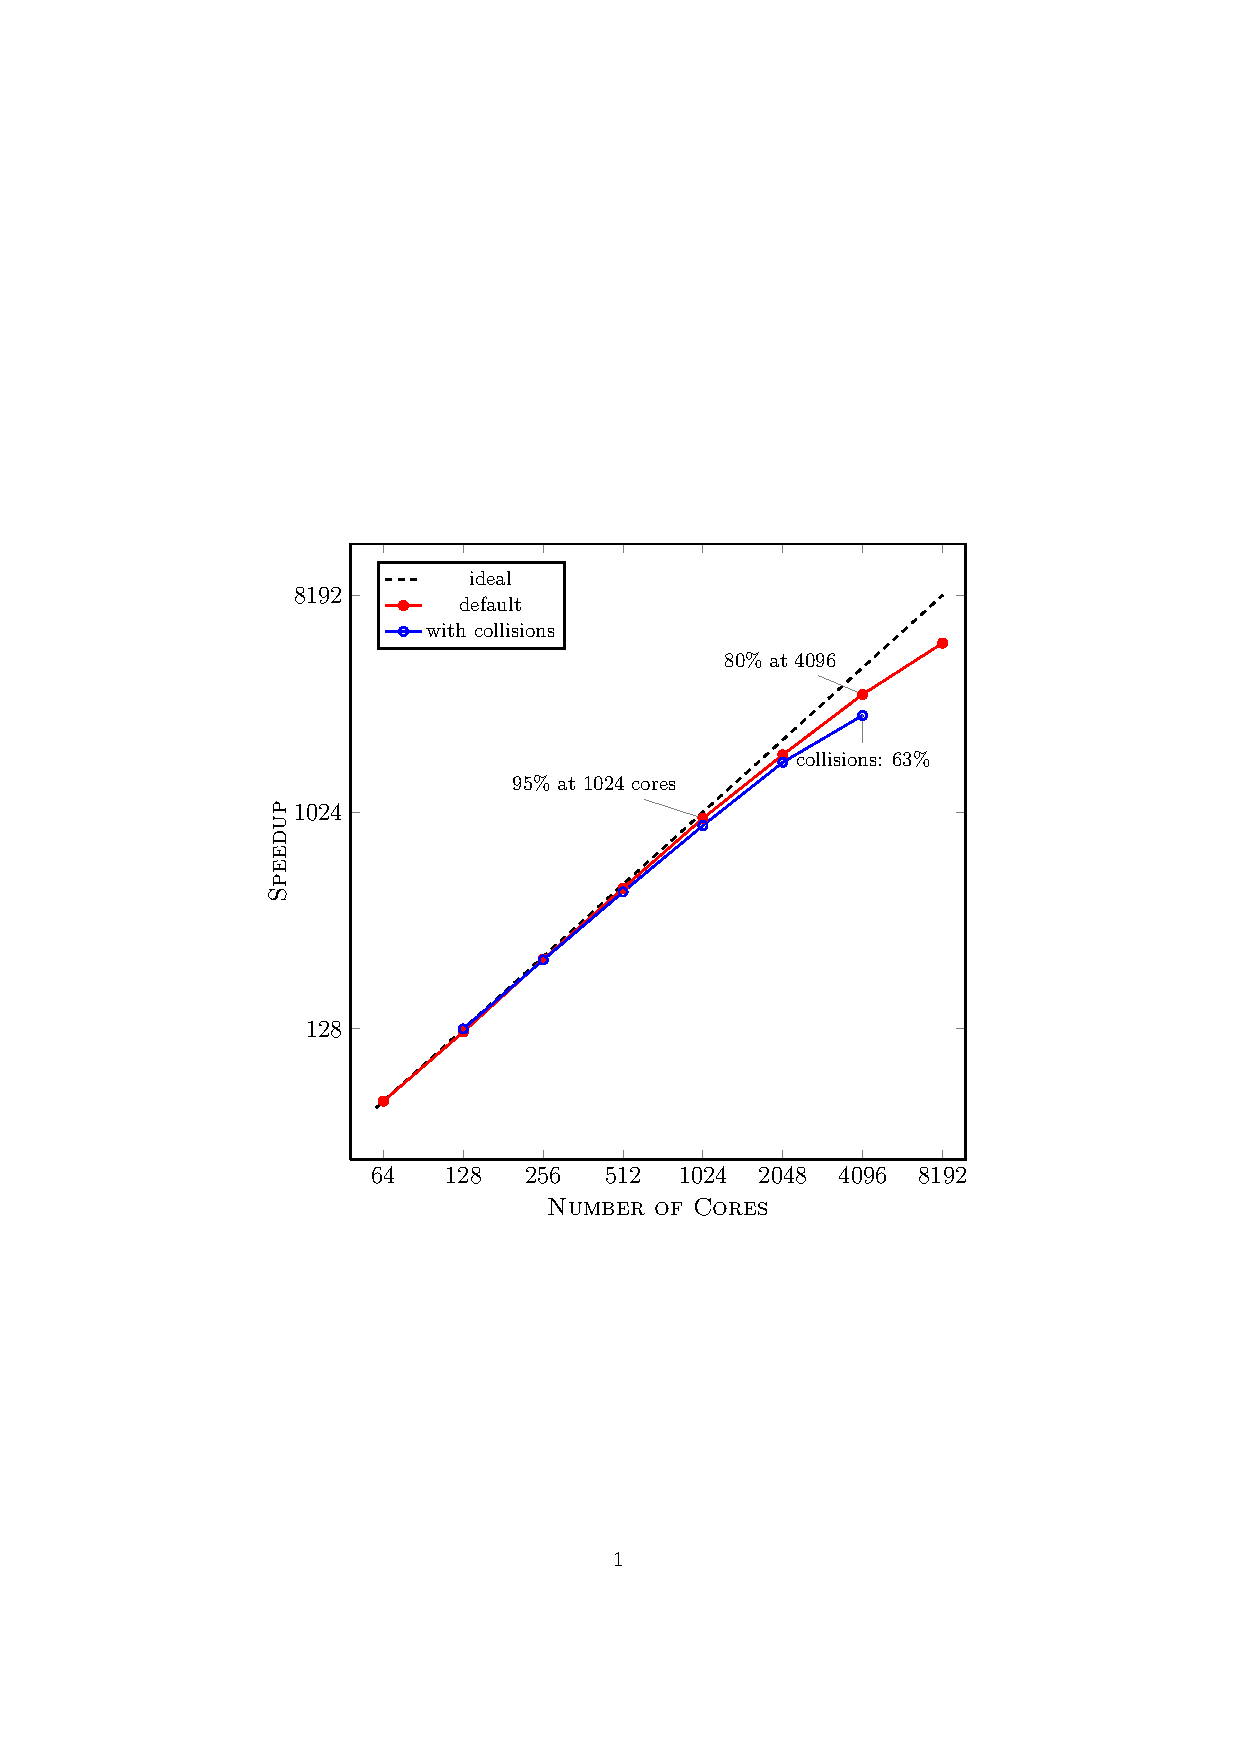
\includegraphics[width=0.5\textwidth,clip]{performance}
\caption{
  Parallel performance for a typical sized problem on HECToR (Cray XT4), both without and 
  with the collision operator turned on. Due to machine memory constraints, this problem can run with
  a minimum of 64 cores without collisions and 128 cores with. The performance/speedup is based on the
  time taken to perform the main time integration loop of the code and is scaled such that it is equal
  to the number of cores when the smallest possible number of cores is used. The parallel efficiency,
  based on $100$\% for the smallest number of cores, is noted at several points on the plot.
}
\label{scaling}
\end{center}
\end{figure}
Here we make a simple assessment of the parallel performance of the code on a Cray XT4 (HECTOR). We define the performance
as the amount of main time loop computation done by the code per unit time. In the ideal case, a doubling in the
number of processor cores used will double the amount of computation done per unit time (or halve the time required
to do a fixed number of time steps).
We consider a non linear problem of fairly typical size that we believe to be reasonably well converged with respect to grid
resolution. As mentioned in Sect.~\ref{memorylayout}, we can change the data memory layout to potentially
tweak the parallelisation and cache efficiency of the code. We have experienced some variation in performance due to these
adjustments. However, we do not yet have enough experience of how to optimally prescribe the layout depending on grid size and parallelisation options,
so for the purpose of this test, we keep the layout fixed to the default. We perform a test with a resolution of 83 radial wave vectors, 21 bi-normal modes, 4 species, 16 $s$ grid points, 16 $\mu$ grid points and 64 $v_\parallel$ grid
points, using fourth-order finite-differences in double precision. Two cases are considered, one using the collision operator and one
without. Due to the memory available per processor core, a minimum of 64 processors are required for the former case and 128 for the latter. 
Using a second-order finite-difference scheme and/or a single precision calculation can reduce this minimum. From the parallel algorithm
perspective, the upper limit on the number of parallel processes used for this case is 16384. Using second-order finite differences would increase this maximum to 65536 cores.
However, only up to 8192 cores were available on the hardware at the time of testing.

Before deciding how to producing a scaling plot for this testcase (such as in Fig.~\ref{scaling}), some preliminary investigations on
the effects of parallelising in each direction were made. Using the `trivial' directions alone, the test case parallelises over the minimum
64 processors for the default case. The difference in performance
between this parallelisation and parallelising primarily over the parallel velocity grid is fairly small, the `trivial' directions giving
less than $10$\% better performance than with the $v_\parallel$ direction. Parallelising primarily over the $s$ grid at
64 cores (using the maximum number of cores in the $s$ direction before using the simple direction) yields a performance which is almost identical
to that using only the `trivial' directions. It seems that for 64 processors, the communication needed for the derivatives has little (if any) effect
on the parallel performance. To get an idea of the relative expense of parallelising over $s$ and $v_\parallel$, two tests were made by starting with 64
cores (using only the trivial parallelisations), then varying either the number of processors in the $v_\parallel$ direction
or the $s$ direction until a total of 512 cores were used. The reduction in efficiency with increasing processors was greater with $v_\parallel$, with the $s$
parallelisation performing around $6\%$ better at 512 cores (at $>95\%$ of the efficiency at 64 processors).

A scaling test was performed for the collisionless case up to 8192 cores. Fig.~\ref{scaling} shows how the performance increases with the number of cores.
For the first point at 64 cores, only the `trivial' directions are used for the parallelisation, since that combination provides the best performance 
(but only by around $1\%$). Since the $s$ direction is the preferred parallelisation direction (least expensive in terms of performance), the number of 
processors in $s$ doubled between each point on the graph up to 512 cores, where the maximum of 8 processors in $s$ is used. Beyond that point, the more expensive $v_\parallel$ grid is decomposed until
8192 cores are used. At 8192 cores, the code runs at $63\%$ of the efficiency at 64 cores.

Following the discussion in the previous subsections, we should expect that with collisions, parallelisation over the $\mu$ direction
is more expensive than over the $s$ direction. Therefore, the scaling test for collisions (as shown in Fig.~\ref{scaling}) starts at 128 processors fully parallelised over the $s$ direction
and over the species, using only 4 processors in $\mu$. Then, the number of processors in $\mu$ is doubled, until 512 cores are used. At 1024 cores, it is cheaper to use 32
processors in $v_\parallel$ and only $1$ in $\mu$, since this avoids using parallelisation in both those directions together. For the final 2 points on the graph, the 
number of processors in the $v_\parallel$ and $\mu$ are either identical, or there are twice as many in $v_\parallel$. Since these
parallelisation combinations give the best performance (considerably better than using the same ones as without collisions), careful consideration should be given to
the number of processors used in each direction when using collisions. At 4096 cores the efficiency is $63\%$ of that at 64 cores.

In both cases considered we see decreasing performance gains when we begin to parallelise in
less favourable directions. Running the tests in single precision would mean less data communicated, so may improve
scaling (but at the same time would likely reduce the time between communication, or the time available for overlapping communication with computation). Running with the second
order finite difference scheme would allow double the number of cores in the $s$ direction and may improve the efficiency
at a large number of cores. If different test cases are considered, it may well be that more resolution in a particular direction
is needed, which would then lend itself to further scaling.

% Something about cartesian topology ordering
For hardware in which not all processor interconnects are equal in speed, the ordering of the MPI communicators within the cartesian topology 
can have a significant effect on parallel performance.  Current high performance machines appear with multiple shared memory cores on interconnected nodes are one example.  Given the above discussion of the bottleneck in global reduction operations, it is preferable that the $s$ direction decomposition should be over the slowest communication direction.  The GKW default setup assumes that MPI rank ordering is done with adjacent physical processors adjacent in the rank ordering.  Testing of a collisionless case on a Cray XT6 (HECTOR phase-2b with 24 cores per node) with 1344 cores indicated that the default dimension ordering (Species, $\mu$, $v_\parallel$, $s$) was optimal.  The configuration ($v_\parallel$, Species, $\mu$, $s$), was 30\% slower, even with exact multiples of the $v_\parallel$ grid (presumably) on a single node.  This is counter-intuitive, since one would expect putting the $v_\parallel$ direction first to be optimal. Configurations with $s$ first were up to 80\% slower. The ordering can be simply reconfigured near the top of \File{grid.F90}.  The optimal configuration will depend on hardware and problem size, and conducting tests prior to expensive runs is recommended.


\section{Parallel performance (hybrid, MPI+OpenMP), BlueGene/P \label{sec:bluegene}}
The performance of pure MPI parallelisation has also been compared to hybrid parallelisation MPI+OpenMP (see Sec.~\ref{sec:hybrid} for details on the hybrid scheme) for a typical non-linear electromagnetic case with kinetic electrons. The problem size is almost the same as in the previous section: 83 radial wave vectors, 20 bi-normal modes, 4 species, 32 $s$ grid points, 8 $\mu$ grid points and 64 $v_\parallel$ grid. A case without collisions and a case with collisions ($R_\textrm{ref}=3$, $T_\textrm{2}$ and $n_\textrm{ref}=6$, was investigated.  In contrast to the previous section, the full collision operator \textit{with} mass and momentum conservation was used\footnote{How much the scaling is affected by the communication required for the momentum conservation has not yet been fully investigated by comparisons on the same machine. Limited tests on BABEL indicated that momentum conservation caused a consistent 4\% slowdown up to 4096 cores, but it could become more (or less) important at higher number of cores (note that it is overlapped with derivatives communications when the MPI implementation supports this).  The version of GKW tested on BABEL did not yet have OpenMP implemented in the calculation of the momentum conserving field. Comparison of timings for the regular fields indicate that implementing this would give a 4\% (2\%) speedup at 4 (2) threads without MPI, but with MPI it will likely make no difference if the scaling bottleneck is in the overlapped derivatives communication.}.

The tests were conducted on the BlueGene/P BABEL (4 cores at 850MHz and 2GB of memory per node \url{http://www.idris.fr/eng/User_Support/bg_support.html}) for which the number of OpenMP threads per node can be 1, 2 or 4. The executable was compiled from revision 2076 of GKW source with O4 optimisation level (typically $10\%$ faster that O2/O3 optimisation for a compilation without OpenMP and $5\%$ faster for a compilation with OpenMP) and double precision. Due to the small amount of memory per node available on BABEL at least 512 cores were required to run the problem under consideration (to be accurate, the run fits on 256 cores but the execution is then very slow). For all the runs in this section, the number of MPI processes in the species and $s$ direction was \name{n_procs_sp}=4 and \name{n_procs_s}=16, respectively. The number of processes in the $\mu$ direction was \name{n_procs_mu}=8 for the collisionless case and \name{n_procs_mu}=4 for the case with collisions (except when 4 threads were used at 512 cores where \name{n_procs_mu} was reduced to 4 and 2, respectively). This means that the MPI parallelisation over the three most favorable directions was maximised to start with and the scaling of the least favorable direction, $v_\parallel$, was then compared to the OpenMP scaling by increasing either \name{n_procs_vpar} or the number of threads per node. For instance, a collisonless run on 2048 cores was performed on 1 thread with \name{n_procs_vpar}=4 or on 2 threads with \name{n_procs_vpar}=2.  The tests were conducted with a typical set of diagnostics with NAVERAGE=100, and with the nonlinear timestep estimator on, both were found to have little effect on the scaling performance (for the single threaded case at least).

The results of the tests are summarised in Table~\ref{table:nocol} (no collisions) and Table~\ref{table:col} (with collisions). The corresponding speed-up and total main loop time is displayed in Fig.~\ref{scalingBABEL} and \ref{scalingBABEL:total}, respectively. Hybrid parallelism with 4 threads is especially useful with collisions and allows to recover the scaling obtained without collisions near the MPI limits. 
\begin{table}
\begin{center}
\begin{tabular}{|c|c|c|c|c|c|c|}
\hline
cores & 512 & 1024 & 2048 & 4096 & 8192 & 16384\\
\hline
1 thread - no OMP& 203.5h & 212.8h & 227.9h& 255.3h & 304.3h & 408.4h \\
(time, efficiency) & 100\% & 95.6\%  & 89.3\%  & 79.7\%&66.9\% & 49.8\%\\
\hline
1 thread & 214.4h & 222.1h & 237.0h& 263.6h & 316.6h & 551.0h \\
(time, efficiency) & 100\% & 96.5\%  & 90.5\%  & 81.3\%& 67.7\% & 38.9\%\\
\hline
2 threads &221.1h & 225.5h & 233.3h& 255.1h & 313.2h & 493.1h \\
(time, efficiency) & 100\% & 98.0\%  & 94.8\%  & 86.7\% & 70.6\% & 44.8\%\\
\hline
\end{tabular}
\caption{Case without collisions. Total main loop time (in hours) for 600 time steps and strong scaling efficiency based on the case with 512 cores.}
\label{table:nocol}
\end{center}
\end{table}
Compilation without OpenMP is slightly faster (due to different cache efficiencies in the matrix ordering). This was also observed on HECTOR. (This has since been changed, both now use the same sort ordering so there is no longer any cache penalty for openmp)
\begin{small}
\begin{table}
\begin{center}
\begin{tabular}{|c|c|c|c|c|c|c|}
\hline
cores & 512 & 1024 & 2048 & 4096 & 8192 & 16384\\
\hline
1 thread& - & 290.0h & 317.9h & 373.1h & 519.2h & - \\
(time, efficiency) & (100\%) & (92.6\%)  & (84.4\%)  & (71.9\%)& (51.7\%) & - \\
\hline
2 threads & 268.4h & 283.0h & 300.4h& 323.4h & 480.6h & 713.6h \\
(time, efficiency) & 100\% & 94.8\%  & 89.4\%  & 83.0\%& 55.9\% & 37.6\%\\
\hline
4 threads & 281.7h & 283.5h & 294.9h & 314.6h & 380.5h & 506.1h \\
(time, efficiency) & 100\% & 99.4\%  & 95.5\%  & 89.5\% & 74.0\% & 55.7\%\\
\hline
\end{tabular}
\caption{Case with collisions (including momentum conservation). Total main loop time (in hours) for 600 time steps and strong scaling efficiency based on the case with 512 cores. On 1 thread, the run at 512 cores was out of memory and the strong scaling efficiency was calculated using the results on 2 threads. }
\label{table:col}
\end{center}
\end{table}
\end{small}

\begin{figure}
\begin{center}
\includegraphics[width=0.4\textwidth]{speedupnocollisions.eps}%
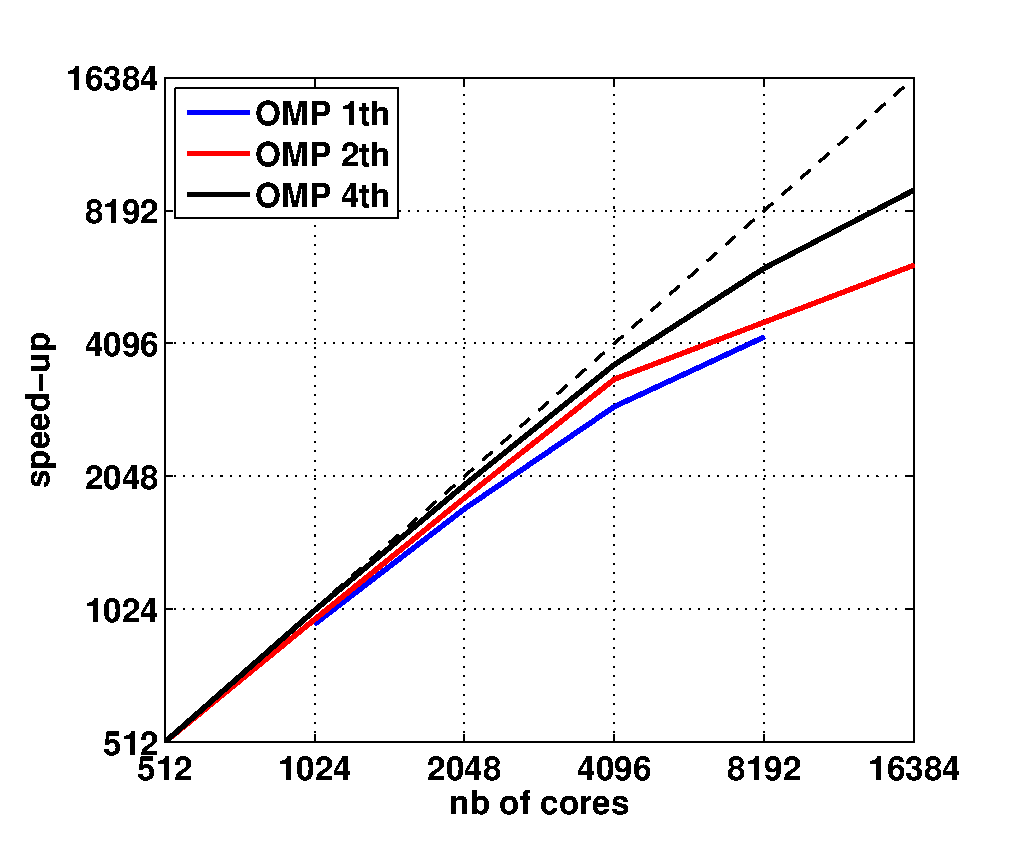
\includegraphics[width=0.4\textwidth]{speedupcollisions.eps}
\caption{ Parallel performance for a typical sized problem on BABEL (BlueGene/P), both without (left plot) and 
  with (right plot) the collision operator (with momentum conservation) turned on. The performance/speedup is based on the
  time taken to perform the main time integration loop of the code and is scaled such that it is equal
  to the number of cores when the smallest possible number of cores is used.}
\label{scalingBABEL}
\end{center}
\end{figure}
\begin{figure}
\begin{center}
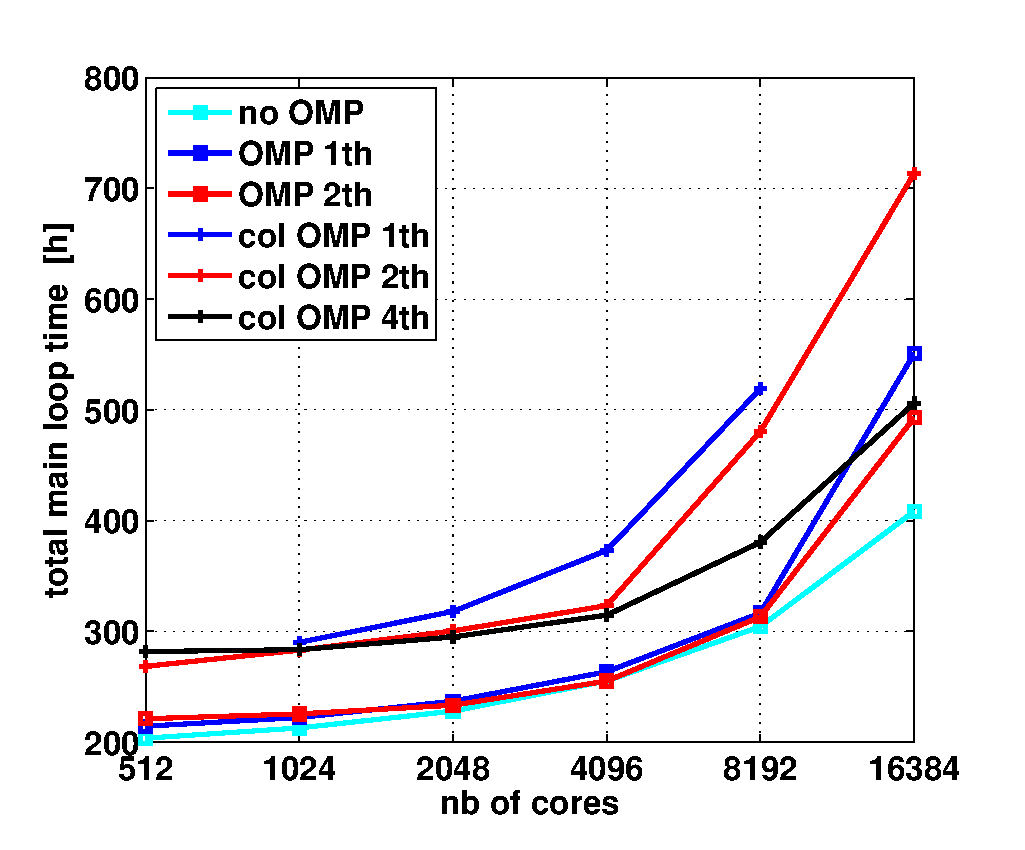
\includegraphics[width=0.5\textwidth]{totaltime.eps}
\caption{ Total main loop time in hours for the cases studied in this section.}
\label{scalingBABEL:total}
\end{center}
\end{figure}

A test has also been performed with the number of modes increased to NX=183 and NMOD=32 with the results summarised in Table~\ref{table:bigcol}.
\begin{small}
\begin{table}
\begin{center}
\begin{tabular}{|c|c|c|c|c|}
\hline
cores & 2048 & 4096 & 8192 & 16384\\
\hline
1 thread& 1166.4h & 1369.1h & 1731.7 h & - \\
(time, efficiency) & 100\% & 85.2\%  & 67.4\%  & -\\
\hline
2 threads & 1094.9h& 1164.4h & 1412.5h & 2317.3h \\
(time, efficiency) & 100\% & 94.0\%& 77.5\% & 47.3\%\\
\hline
4 threads &1081.7h & 1136.5h & 1305.4h & 1692.5h \\
(time, efficiency) & 100\% & 95.2\% & 82.9\% & 63.9\%\\
\hline
\end{tabular}
\caption{Case with collisions (with momentum conservation), NX=167 and NMOD=32. Total main loop time (in hours) for 600 time steps and strong scaling efficiency based on the case with 2048 cores. }
\label{table:bigcol}
\end{center}
\end{table}
\end{small}

\pagebreak


\section{Parallel nonspectral performance (pure MPI), Helios}

The nonspectral version of the code additionally parallelizes over the radial (x) direction (with the exception an implicit solve for the polarization term).  The nonspectral 
version of the code spends proportionally more time in the fields calculations than the spectral version, since the multi-point averages use for the gyroaverages are much slower 
than the Bessel functions of the spectral version. (The nonlinear terms, by contrast, are much faster since they only require 1D FFTs.)

Since the ``diagonal part'' of the fields solve is only 3 dimensional, it cannot parallelise over the velocity space or species.   This is true in both the spectral and nonspectral
versions, but in the spectral version, the diagonal part of the fields solve takes a neglible of CPU time.  To allow efficient scaling for the nonspectral version, the fields solve 
work is additionally parallelised over the toroidal modes using the same communicators that are elsewhere used to distribute work over the velocity space and species. 
This feature also reduces the fraction of time spent in the implicit polarization solve, which is radially global. Two allgather communications are therefore required in the fields
solve: The first in x before the polarization solve, and the second in nmod after the polarization solve so that every processor obtains the result for every toroidal mode. 
Since these are both gather operations of 3d quantities, they are relatively fast compared to the reductions and communications of ghost cells.  

Parallelization over the x direction brings the same benefits for reducing the reduction operations in the field solve as the parallelism over the s direction. The additional
penalties of extra ghost cell and allgather communications in the fields solve are outweighed by the benefit that this brings.  The result is that parallelism over x is always more
efficient than parallelism over parallel velocity (which in the nonspectral case performs much worse than in the spectral case due to the larger fraction of time in the field
solve).  For more details see \raw{doc/GKW_MPI_nonspectral.pdf}.

Scaling tests of the radially nonspectral version of the code (Fig. \ref{scalingHelios}) were performed on the Bull IFERC Helios machine (Intel Sandy Bridge with fat tree topology Infiniband
communication network).  As with the scaling test described in Sec. \ref{scaling-orig}, the `trivial' parallel directions were used first, followed by s, then x (although not to maximum), then finally vpar.
Two cases were chosen to represent a medium and a large physics case simulation, with gridsizes
\begin{verbatim}
NX = 256, N_s_grid = 32,  N_mu_grid = 16,  N_vpar_grid = 32,  NMOD = 16, number_of_species = 2
\end{verbatim}
for the medium case, and 
\begin{verbatim}
NX = 512, N_s_grid = 64,  N_mu_grid = 16,  N_vpar_grid = 64,  NMOD = 43, number_of_species = 2
\end{verbatim}
for the large case.

The radial box size was \texttt{lx = 128} or \texttt{lx = 256} respectively, which resulted in 6 x ghost points required for the gyroaverages (only two are communicated for the derivatives).  Since the number of ghost points must be less than the number of local points, this sets the maximum limit of \texttt{n_procs_x = 32} or \texttt{64} repsectively.

\begin{figure}[htb!]
\begin{center}
\includegraphics[width=0.48\textwidth]{scaling-helios-med3}
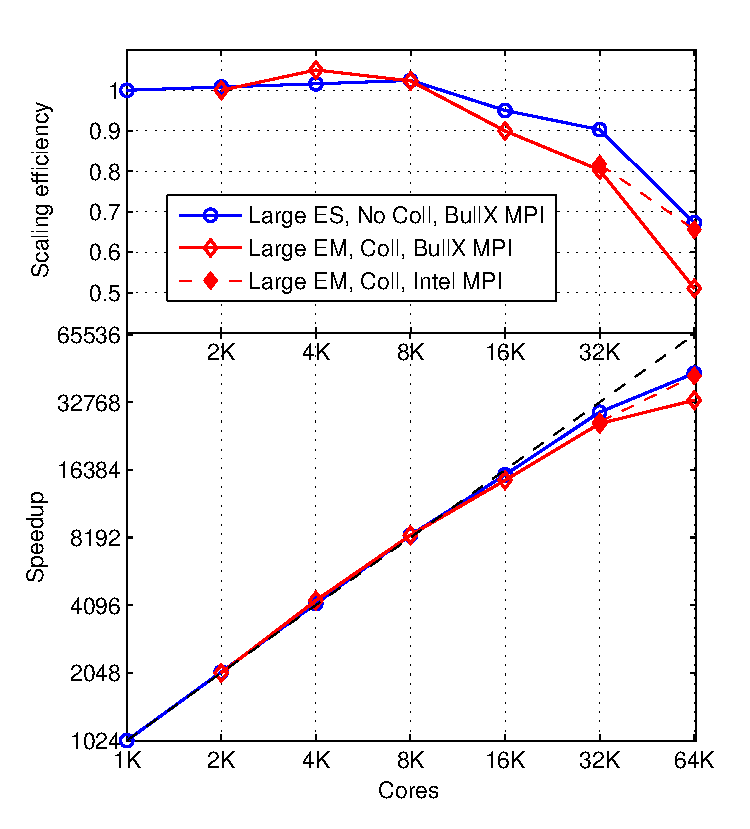
\includegraphics[width=0.49\textwidth]{scaling-helios-large3}
\caption{ Strong scaling performance for the medium and large sized nonspectral problems on Helios. 
          The speedup is based on the time taken to perform the main time integration loop 
          of the code and is scaled such that it is equal to the number of cores when the smallest possible number of cores is used.
          BullX MPI seems to perform better at ghost cell communications of derived datatypes while Intel MPI seems to perform better at the large
collective operations.  Which is better therefore depends on which MPI communication is dominant for a given problem.}  
\label{scalingHelios}
\end{center}
\end{figure}

For the medium problem size, the maximum possible \texttt{n_procs_x=32, n_procs_vpar=16} would allow a theoretical maximum of 131,072 cores (65,536 with collisions).  For the large problem size, the maximum possible \texttt{n_procs_x=64, n_procs_vpar=32} allows a theortical maximum of 1,048,576 cores (524,288 with collisions).  These results compare favorably with the spectral scaling tests: 
The parallelism over x removes any scaling performance penalty associated with the use of the collision operator
(which adds 20\% to all runtimes).  



% related to auctex mode and latex-preview-mode in Emacs:
%%% Local Variables:
%%% mode: latex
%%% TeX-master: "doc"
%%% End:
